\chapter{Elementi di economia d'impresa}
L'economia si divide in due:
\begin{itemize}
    \item \textbf{economia aziendale}: studia la differenza fra aziende e il loro funzionamento interno
    \item \textbf{economia politica}: studia i problemi di equilibrio del sistema politico
\end{itemize}

\section{Economia aziendale}
\begin{quotation}
    ``Disciplina che studia le condizioni di esistenza e le manifestazioni di vita dell'azienda.''

    G. Zappa
\end{quotation}

Incentrata sull'azienda vista come ordine economico di un istituto sociale:
\begin{itemize}
    \item famiglia
    \item impresa
    \item ente pubblico
    \item istituto no profit
\end{itemize}

Ne illustra diversi problemi connessi al funzionamento, con l'obbiettivo di disporre di una base conoscitiva
per guidare le decisioni.

Studia in maniera integrata:
\begin{itemize}
	\item l'organizzazione aziendale: studio dei fattori interni all'azienda e dei rapporti tra azienda
		e ambiente.
	\item la gestione aziendale: operazioni interne ed esterne che creano reddito e variano il capitale.
	\item rilevazione di fatti economici: inventari, preventivi, registrazione di gestione, bilancio di esercizio,
		ecc
\end{itemize}

\section{Definizione di azienda}
deriva dallo spagnolo che deriva dal latino "facienda"(le cose da farsi).

\section{Definizione giuridica di azienda}
\textbf{Complesso di beni organizzati dall'impreditore per l'esercizio dell'impresa.}
Strumenti attravero il quale l'impreditore svolge attività di impresa.


\textbf{È imprenditore chi esercita profesionalmente una attività economica organizzata al fine della
produzione e scambio di beni o servizi}.

\subsection{Caratteristiche impresa}
\begin{itemize}
	\item è attività: serie di atti diretti alla produzione o allo scambio di beni/servizi
	\item è attività economica: deve essere organizzata di modo che i costi siano inferiori ai ricavi
	\item è attività organizzata: per organizzazione si intende l'organizzazione di fattori produttivi(
		capitale, lavoro, macchinari, ecc)
	\item è attività professionale: esercizio svolto con continuità, determinazione intenzionalità
\end{itemize}

\subsection{Caratteristiche azienda}
\begin{itemize}
	\item apparato strutturale(locali, macchine, materie, ecc) di cui l'impresa si avvale.
\end{itemize}


\section{Definizione economico-aziendale di azienda}

L'azienda è:\begin{quotation}
    `` un istituto economico destinato a perdurare che,
per il soddisfacimento dei bisogni umani, ordina e svolge in
continua coordinazione la produzione o il procacciamento e il
consumo della ricchezza. ''

G. Zappa
\end{quotation}

\begin{quotation}
    `` un sistema di forze economiche che sviluppa,
    nell’ambiente di cui è parte complementare, un processo di
    produzione, o di consumo, o di produzione e di consumo
    insieme, a favore del soggetto economico, ed altresì degli
    individui che vi cooperano ''

A. Amaduzzi
\end{quotation}

\subsection{Caratteristiche di un azienda(economico-aziendale)}

\begin{itemize}
    \item organizzazione stabile, per coordinare e combinare il processo produttivo
    \item persone, che prestano le loro energie coordinandosi
    \item beni econimici, materiale, macchine, soldi, destinati ad essere utilizzati
    \item oggetto aziendale, attività svolta
    \item operazioni, sui beni svolto dalle persone per adempiere al fine dell'azienda
    \item fine(scopo)
    \item visione sistematica:
    i fatti aziendali non sono tra loro scollegati, tutto legato da causa effetto.
    \item autonomia:
    liberta di decisione (livello strategico, operativo)
    \item economicità: l'attività deve essere sempre ispirata alla logica:
    \begin{itemize}
        \item efficacia strategica: programmare e realizzare gli obiettivi
        \item efficacia operativa: realizzare la produzione a dovuti livelli qulitativi
    \end{itemize}
\end{itemize}


\section{Azienda come sistema aperto}

Per opravvivere l'azienda deve continuamente intrattenere continue relazioni di scambio con altre entità.


\section{Azienda come sistema socio-tecnico}

L’azienda è un sistema sociale all’interno del quale
operano risorse umane e tecniche (mezzi di produzione)
scarse (caratterizzate, cioè, da una disponibilità limitata),
organizzate e finalizzate al profitto.

\section{Impresa come sistema cognitivo}

La vera ricchezza dell'impresa è legata a:
\begin{itemize}
    \item immagine positiva
    \item avviamento sul mercato
    \item capacità di innovare
\end{itemize}

La conoscenza presente in azienda deriva direttamente sul campo(learnign bt doing)
e indirettamente dalle persone che operano nell'organizzazione.

La visione cognitiva porta a mettere il focus sul la to 
non materiale dell'impresa.

\section{L'imprenditore}
Solitamente quando si pensa a ``imprenditore'' si pensa 
alla definizione di \textbf{imprenditore commerciale}, ma essite anche 
l'\textbf{imprenditore agricolo}.

Limprenditore agricolo(art. 2135 c.c.) produce coltivazioni animali ecc,
l'imprenditore commerciale(art. 2195 c.c.) pensa alla produzione 
di beni e/o servizi, fa da intermediari nella circolazione
dei beni, trasporto, banca, attività ausiliare.

Il soggetto che esercità l'attività commerciale può essere sia singolo(impenditore individuale)
che un gruppo di individui(impenditore commerciale).

\section{Soggetto giuridico e soggetto economico}

\subsection{Soggetto giuridico}
persona fisica o giuridica che assume i diritti 
e gli obblighi derivati dalle operazioni aziendali.

\subsection{Soggetto economico}
persona o gruppo di persone che controlla l'azienda,
influenza le scelte e trae i maggiori vantaggi.

È il soggetto che gode degli utili dell'azienda e ne supporta le perdite.

\section{Stakeholders aziendali}
\begin{figure}[h!]
    \centering
    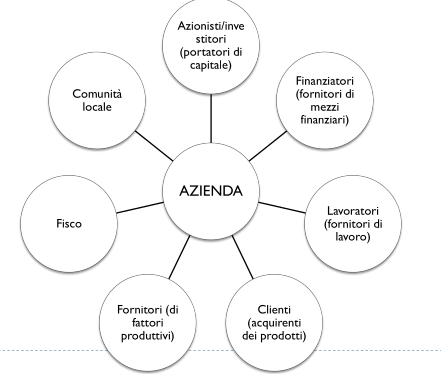
\includegraphics[width=0.5\linewidth]{img/2022-03-27-11-53-12.png}
    \label{fig:stackeholders}
    \caption{Stackeholders aziendali}
\end{figure}
\subsection{Attese degli stakeholders}
\begin{itemize}
    \item \textbf{azionisti - soci - investitori}: profitti, diidenti, controllo
    \item \textbf{finanziatori}: quota capitale, benefit
    \item \textbf{lavoratori}: salario, stipendio, benefit
    \item \textbf{clienti}: rapporto qualità prezzo
    \item \textbf{fornitori}: corrispettivi delle forniture, stabilità, tempi
    \item \textbf{fisco}: imposte, tasse
    \item \textbf{comunità locale}: responsavilità sociale
\end{itemize}
\pagebreak


\section{Classificazione dell'azienda}

\begin{figure}[h!]
    \centering
    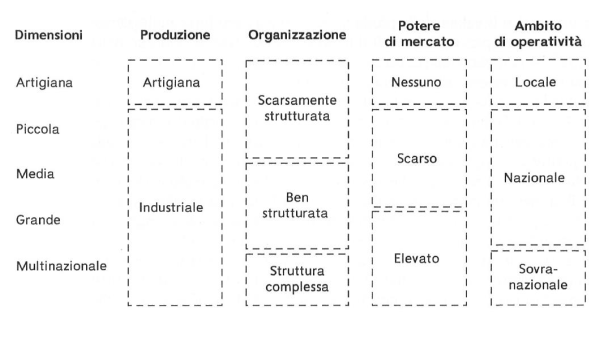
\includegraphics[width=0.5\linewidth]{img/2022-03-27-12-02-19.png}
    \label{fig:classificazione_aziendale}
    \caption{Classificazione aziendale}
\end{figure}
\subsection{Scopo}
\begin{itemize}
    \item produzione
    \item erogazione
    \item composte/miste
\end{itemize}
\subsection{Soggetto giuridico}
\begin{itemize}
    \item azienda publiche (o amministrazione pubblica)
    \item azienda private:
    \begin{itemize}
        \item azienda non profit
        \item azienda for profit
    \end{itemize}
\end{itemize}
\subsection{Forma giuridica}
\begin{itemize}
    \item aziende individuali
    \item aziende collettive o societarie:
    \begin{itemize}
        \item società di persone
        \item società di capitali
    \end{itemize}
\end{itemize}
\subsection{Settore di attività}
Settore:
\begin{itemize}
    \item primario
    \item secondario
    \item terziario
    \item quaternario(terziario avanzato)
\end{itemize}
\subsection{Dimensioni}
\begin{itemize}
    \item grandi
    \item medie
    \item piccole
\end{itemize}
\subsection{Mercato}
\begin{itemize}
    \item Mercato concorrenziale
    \item Mercato non concorrenziale
\end{itemize}
\subsection{Localizzazione dei mercati di vendità}


\begin{itemize}
    \item locale
    \item nazionale
    \item multinazionale
\end{itemize}

\subsection{Azienda individuale}
La proprietà di mezzi di produzione e l'attività fanno a capo ad 
una sola persona fisica(imprenditore).

\begin{itemize}
    \item no autonomia patrimoniale
    \item se fallisce l'azienda, fallisce l'imprenditore
\end{itemize}

\subsection{Azienda collettiva}
Duo o più soggetti dietro ai capitali, dividendo cosi il rischio 
e porfitti.

\subsection{Società}
\begin{quotation}
    ``con il contratto di Società due o più persone conferiscono beni
    o servizi per l’esercizio in comune di una attività economica
    allo scopo di dividerne gli utili (art. 2247 c.c.).''
\end{quotation}

\begin{itemize}
    \item deve essere stipulata tra due o più soggetti
    \item prevede il conferimento di risorse per l'esercizio in comune dell'attività economica
    \item responsabilità e rischio dei soci possono essere limitati alla quota da ciascuno conferita
    \item il potere di amministrazione può essere dissociato dalla qualità di socio
    \item la qualità di socio può essere liberamente trasferibile
\end{itemize}

\section{Forme giuridiche d'impresa}
\begin{figure}[h!]
    \centering
    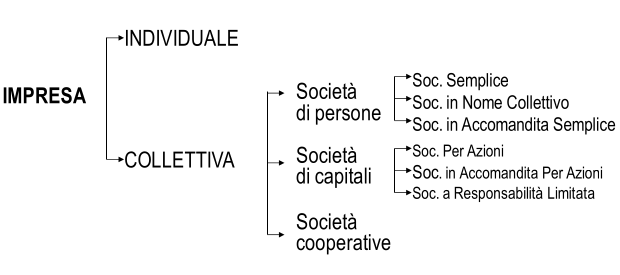
\includegraphics[width=0.6\linewidth]{img/2022-03-27-19-09-18.png}
\end{figure}

\subsection{Società di persone VS capitali}
Nelle società di persone prevalgono i soci sul capitale, viceversa per le società di capitali.

\begin{itemize}
    \item autonomia patrimoniale
    \begin{itemize}
        \item imperfetta per società di persone perchè il patrimonio della società non è perfettamente
        distinto da quello dei soci
        \item peprfetta per società di capitali
    \end{itemize}
    \item personalità giuridica
    \begin{itemize}
        \item non riconosciuta per le società di persone
        \item riconosciuta per le società di capitali
    \end{itemize}
    \item potere amministrativo
    \begin{itemize}
        \item congiunto alal qualità di socio nelle società di persone
        \item disgiunto dalle qualità di socio nelle società di capitale
    \end{itemize}
    \item responsabilità dei soci
    \begin{itemize}
        \item limitata per le società di capitale
        \item illimitata(obligazioni sociali tramite apport odel socio e proprietà personale),
         solidale(i creditori possono rivalersi del patrimonio personale di u socio),
         sussidiaria(patrimonio insufficiente a onorare le obbligazio della società) per le società di persone
    \end{itemize}
    \item controllo
    \begin{itemize}
        \item diretto per le società di persone
        \item indiretto per quelle di capitali
    \end{itemize}
\end{itemize}

\section{Società di persone}
\subsection{Società semplice}
\begin{itemize}
    \item impresa piccola o piccolissima
    \item contratto scritto o implicito
    \item modifica ai patti sociali approvati all'unanimità
    \item soci indicati nell'atto costitutivo con i relativi conferimenti
    \item qualità di socio non trasferibile
    \item responsabilità diretta, illimitata e solidale
    \item ripartizione di utili, perdite in proporzione al conferimento
    \item rendiconto annuale di esercizio
    \item sciogliemnto per:
    \begin{itemize}
        \item decorso termine
        \item conseguimento oggetto sociale o impossibilità
        \item volontà unanime dei soci
    \end{itemize}
    \item nessuna dichiarazione di fallimento
    \item liquidazione: pagati i debiti, il residuo si divide fra i soci
\end{itemize}

\subsection{Società in nome collettivo(SNC)}
